\documentclass{article}
\usepackage[utf8]{inputenc}
\usepackage{longtable}
\usepackage{authblk}
\usepackage{adjustbox}
\usepackage{natbib}

\title{CARACTERIZACIÓN DE LOS INDICES DE DESARROLLO HUMANO EN COLOMBIA}
% autores
\renewcommand\Authand{, y }
\author[1]{\normalsize Carolina Barreto Naranjo}
\author[2]{\normalsize Andrea Calderon Corredor}
\author[3]{\normalsize Andrea Blanco Zarta}

\affil[1,2,3]{\small  Facultad de Ingeniería,Universidad de los Andes\\
\texttt{{c.barreto805,a.calderon,a.blanco}@uniandes.edu.co}}
\affil[1,2,3]{\small Herramientas Computacionales para la Investigación\\}

\date{29 de Junio de 2018}

\usepackage{Sweave}
\begin{document}
\Sconcordance{concordance:matriz.tex:matriz.Rnw:%
1 22 1 1 0 37 1}


\maketitle


\begin{abstract}
En este trabajo se hace un análisis de la evolución del IDH como indicador social. Primero se realiza una discusión sobre la importancia de colocar en la agenda social al IDH. Posteriormente se presentan los elementos que componente el IDH. Por último se analizan los indicadores del IDH tanto a nivel global como para México. La desigualdad existe desde los primeros hombres, esta se debe medir y se debería de crear un consenso sobre la forma de medirla y de compararla entre los distintos países, estados y entidades de distinta índole. Al hablar de la igualdad, se debe de tomar en cuenta desde qué “ángulo” estamos viendo la situación, desde la perspectiva del utilitarismo o no.
\end{abstract}

\section*{Introducción}

El Índice de Desarrollo humano (IDH) es un indicador creado por el Programa de las Naciones Unidas para el Desarrollo (PNUD) con el fin de determinar el nivel de desarrollo que tienen los países del mundo.  Fue ideado con el objetivo de conocer, no sólo los ingresos económicos de las personas en un país, sino también para evaluar si el país aporta a sus ciudadanos un ambiente donde puedan desarrollar mejor o peor su proyecto y condiciones de vida. La principal amenaza al progreso en América Latina y El Caribe es la recaída de millones de hogares en la pobreza, pero la ralentización económica no es la única culpable de tal regresión. El informe presenta recomendaciones para que los países de la región -incluido Colombia- impidan retrocesos y siga avanzando en lo social, económico y ambiental, con políticas públicas de nueva generación, en línea con los Objetivos de Desarrollo Sostenible (ODS).
 
Comencemos viendo que hay en la sección \ref{univariada} en la página \pageref{univariada}.

\clearpage

\section{Exploración Univariada}\label{univariada}




Teniendo en cuenta queel estudio se hizo para los 32 departamentos de Colombia

% Table created by stargazer v.5.2.2 by Marek Hlavac, Harvard University. E-mail: hlavac at fas.harvard.edu
% Date and time: vie., jun. 29, 2018 - 7:22:42 p.m.
\begin{table}[!htbp] \centering 
  \caption{Medidas estadísticas} 
  \label{stats} 
\begin{tabular}{@{\extracolsep{5pt}}lccccc} 
\\[-1.8ex]\hline 
\hline \\[-1.8ex] 
Statistic & \multicolumn{1}{c}{Mean} & \multicolumn{1}{c}{Median} & \multicolumn{1}{c}{St. Dev.} & \multicolumn{1}{c}{Min} & \multicolumn{1}{c}{Max} \\ 
\hline \\[-1.8ex] 
IDH & 0.802 & 0.804 & 0.042 & 0.691 & 0.879 \\ 
Poblacion.Cabecera & 1,196,730.000 & 717,197 & 1,982,287.000 & 13,090 & 10,070,801 \\ 
Poblacion.Resto & 360,590.300 & 268,111.5 & 331,887.600 & 21,926 & 1,428,858 \\ 
Poblacion.Total & 1,557,320.000 & 1,028,429 & 2,202,522.000 & 43,446 & 10,985,285 \\ 
\hline \\[-1.8ex] 
\end{tabular} 
\end{table} \centering




\begin{figure}[h]
\centering
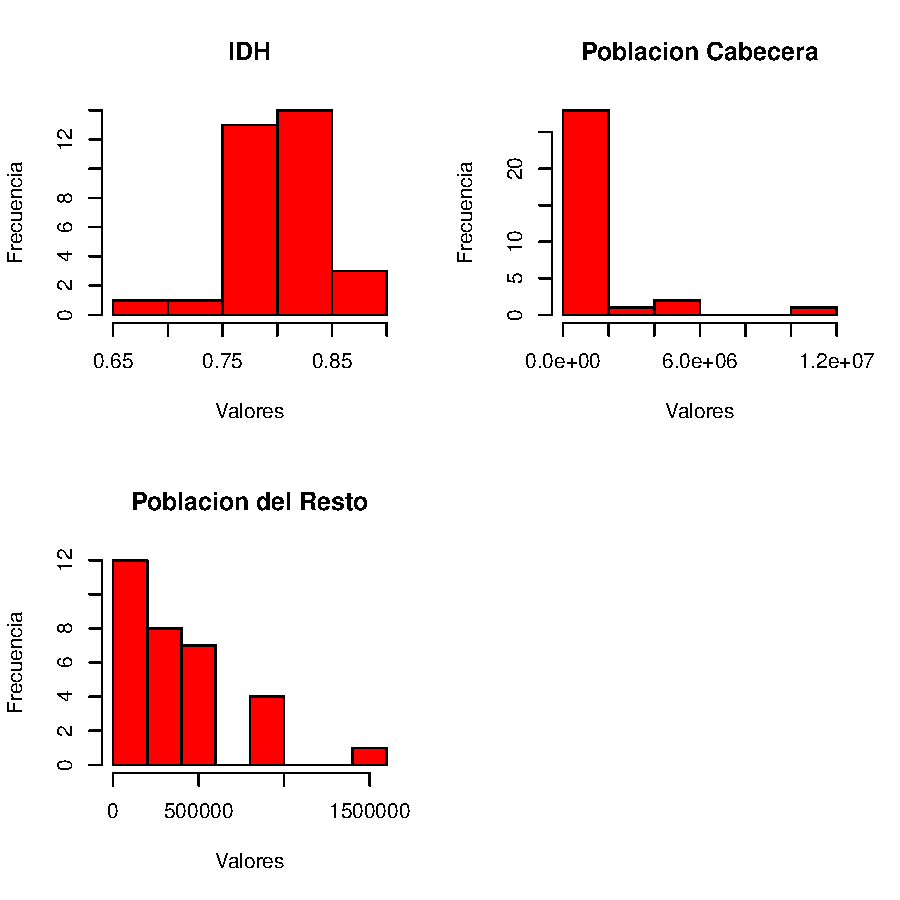
\includegraphics{univariada-hist}
\caption{Distribuci?n de Indicadores}
\label{hist}
\end{figure}

Si quieren normalizar dado el sesgo de las poblaciones, se tranforma con logaritmo en case 10 y quedaria asi:

\begin{figure}[h]
\centering
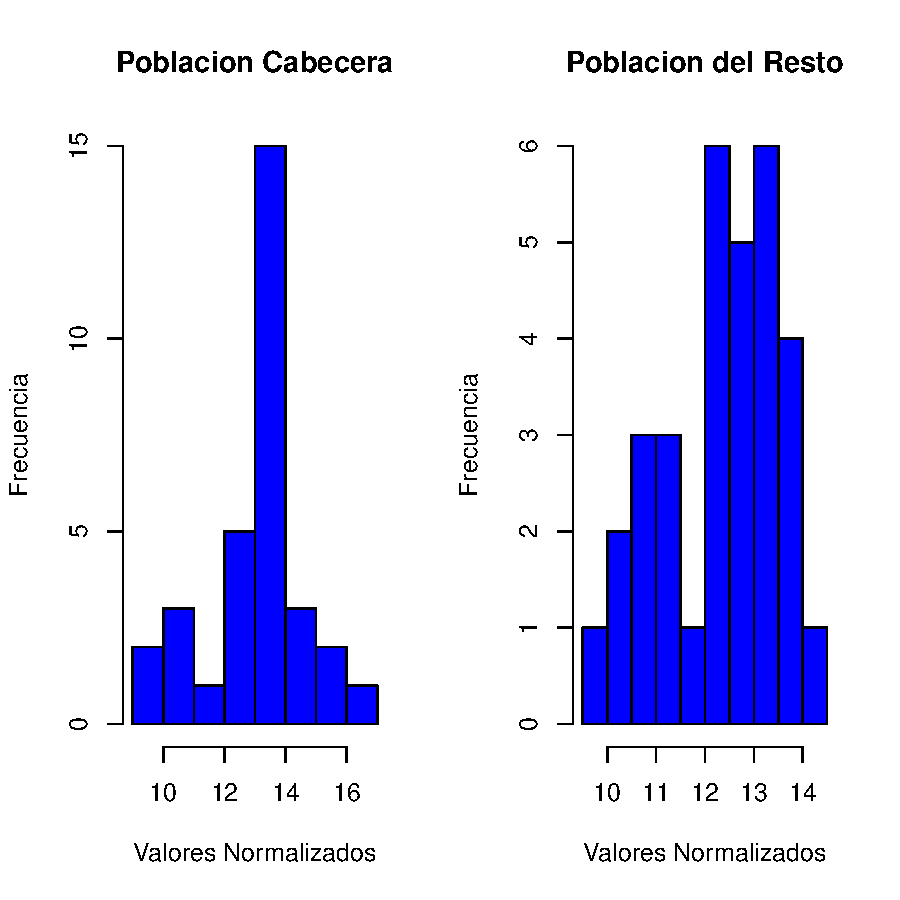
\includegraphics{univariada-hist1}
\caption{Distribuci?n de Indicadores de Poblaciones Normalizado}
\label{hist1}
\end{figure}

\endinput

\section{Exploración Bivariada}\label{bivariada}


Según el Programa de las Naciones Unidas para el Desarrollo (PNUD) Colombia ha mejorado el índice de desarrollo humano por los logros en la cobertura de educación y salud e incrementar el ingreso per cápita. Esto permitió pasar del puesto 77 al 69. Sin embargo, preocupa estar de undécimo entre los países con peor distribución del ingreso; el ingreso de un rico equivale a lo que reciben 58 personas más pobres de Colombia, mientras en Dinamarca y Japón equivale a 24.7 y 24.9 respectivamente.

Una de las mayores barreras para reducir la pobreza es la inequidad distributiva de la riqueza. La sociedad colombiana es pobre, presenta una distribución desigual del ingreso y crece poco. Es probable que una mejor distribución del ingreso facilite el crecimiento económico, que sólo es posible con una base institucional confiable y con políticas macroeconómicas estables enfocadas hacia el desarrollo individual.


\section{Modelos de Regresion}\label{regresion}


En conclusión, vemos los modelos propuestos. Primero sin la poblacion restante como variable independiente, y luego con está. Los resultados se muestran en la Tabla \ref{regresiones} de la página \pageref{regresiones}.


\section{Exploración Espacial}\label{espacial}

La ruta más expedita para salir de la pobreza es el desarrollo humano. Para impulsarlo debe haber acceso a servicios de salud y educación de buena calidad. Si Colombia quiere tener pros-peridad y justicia social, requiere atender la equidad entre sus zonas rurales y urbanas, entre sus regiones, entre grupos étnicos y entre hombres y mujeres en aspectos como el acceso a la educación, la propiedad de la tierra y la distribución del ingreso.


Según la encuesta de salud sexual y reproductiva de PROFAMILIA del año 2005, la sociedad colombiana ha cambiado radicalmente en los últimos 50 años, con descenso de la tasa global de fecundidad de 6.8 a 2.4, el de mortalidad bruta de 16.7 a 5.5 y el de mortalidad infantil de 123.2 a 25.6 (aún vergonzosa). La esperanza de vida de los colombianos aumentó de 50.6 a 72.2 años, pero también son vergonzosas las diferencias regionales y entre estratos sociales. La mortalidad infantil en el Chocó es tan alta como la africana. Hay 10 puntos de diferencia entre la mortalidad infantil urbana y la rural. El problema de desnutrición infantil continúa sin atención y 12% de los niños son desnutridos crónicos.


Nuevos estudios sugieren que el estrés de ser pobre tiene una peligrosa influencia en la salud. Cuando se comparan los estados socioeconómicos altos y bajos, el riesgo de algunas enfermedades es diez veces mayor. Las personas de estrato socioeconómico bajo tienen dramáticamente más riesgo de enfermar y expectativa de vida más corta.



\bibliographystyle{apalike}
\renewcommand{\refname}{Bibliografia}
\bibliography{Colombia}

\end{document}
